\documentclass[10pt]{article}
\usepackage{amsmath,graphicx,booktabs,hyperref}
\usepackage[margin=1.7cm]{geometry}
\graphicspath{{figures/}}
\title{What Drives Performance in AIGC Edited-Region Localization?}
\author{SparseViT experiments, error localisation, \\ and comparison with the historical native-resolution pipeline}
\date{November 2026}
\begin{document}
\maketitle
\section{Executive conclusion}
\textbf{Claim.} Pixel-scale fidelity and full-image, metric-aligned checkpoint selection determine performance here, but a genuinely different architecture adds a second informative signal. The historical native-crop U-Net reached a public Score of $0.92213$ (ref $58415875$), while SparseViT trained on square-downscaled whole images reached $0.65764$. Native $512\times512$ crops raised SparseViT to $0.77279$, and a global/native two-view ensemble reached $0.80870$. A teacher--hard probability fusion with TTA8, overlap 64, and hysteresis postprocessing reached $0.93024$ (ref $58747907$). A Mesorch-style dual-frequency segmentation model with the paper's ImageNet-1K ConvNeXt local backbone was then trained from scratch on the supplied masks and fused with the hard model at equal weight, giving \textbf{0.94005} (ref $58928971$). The top-3 cutoff is $0.95843$; the remaining gap is $0.01838$, with the current entry in sixth place.

The result changes the diagnosis. On the 56-image clean-validation split the earlier teacher/hard fusion scored $0.953140$ (mIoU $0.947178$, recall $0.967050$), while a per-pixel oracle over that family scored only $0.95493$: the family was within $0.00179$ of saturation. Three frozen-DINOv2 variants also failed their gates (Section~\ref{sec:dino}). The gain came instead from a second architecture whose errors are complementary: Mesorch alone scores $0.94712$ on clean validation, and the equal-weight Mesorch/hard fusion reaches $0.95516$, $+0.01044$ over the same-protocol teacher/hard baseline. Section~\ref{sec:mesorch} reports the full result, including why boundary postprocessing and full-resolution probabilities were rejected.

\section{Score progression and the leaderboard}
\begin{table}[htbp]\centering\footnotesize
\caption{Historical public submissions from the native-resolution pipeline.}
\label{tab:hist}
\begin{tabular}{llr}
\toprule Score & Ref & Description \\
\midrule
0.92213 & 58415875 & native-crop family, best \\
0.92114 & 58369543 & native-crop family \\
0.92056 & 58373393 & native-crop family \\
0.91484 & 58346197 & native-crop family \\
0.90638 & 58474337 & EfficientNet-B0 RGB, native 512, epoch 26, single view \\
\bottomrule
\end{tabular}
\end{table}
\begin{table}[htbp]\centering\footnotesize
\caption{Our submissions and the canonical fusion.}
\label{tab:ours}
\begin{tabular}{llrr}
\toprule Version & Method & Threshold & Score \\
\midrule
v1 & Global 512 cache & 0.20 & 0.65764 \\
v2 & Global 512 sliding & 0.16 & 0.61291 \\
v3 & Native 512 patches + sliding & 0.86 & 0.77279 \\
v4 & Equal-weight ensemble & 0.48 & 0.80113 \\
v5 & Weighted ensemble (0.4/0.6) & 0.59 & 0.80870 \\
final & Teacher+hard fusion, TTA8/ov64 & 0.92/0.38 & 0.93024 \\
canonical & Mesorch+hard fusion + consensus gate & 0.92/0.38 & \textbf{0.94005} \\
\bottomrule
\end{tabular}
\end{table}
Two pipeline bugs were identified before the later runs. A five-column upload shaped like \texttt{sample\_submission.csv} returned \texttt{SubmissionStatus.ERROR}; the accepted format is two columns \texttt{ID,Predicted}. Submission v2 thresholded uint8 probability maps without dividing by 255 and predicted almost every pixel as edited. Fig.~\ref{fig:scores} shows the progression.

\begin{figure}[htbp]\centering
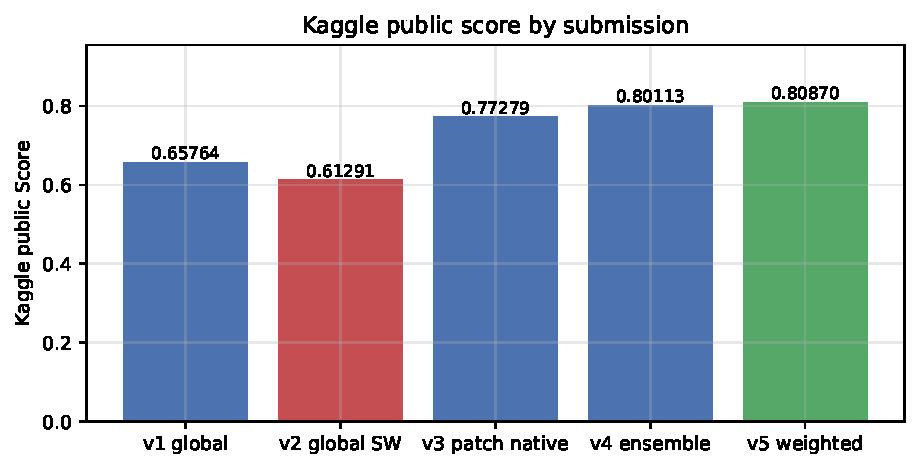
\includegraphics[width=.60\linewidth]{fig_kaggle_scores}
\caption{Kaggle public Score by submission.}
\label{fig:scores}
\end{figure}

\section{Residual errors are local, not global}
On the 500-image validation set used for SparseViT, mean Score falls from $0.8746$ for edits above $5\%$ of pixels to $0.6587$ below $1\%$ and $0.3115$ below $0.1\%$. The global model predicts $1.83$ connected components per image against $4.22$ in the ground truth, with a median component more than twice as large; the native-patch model predicts $4.01$.
\begin{table}[htbp]\centering\footnotesize
\caption{Connected-component structure on validation masks (mean per image; ``tiny'' $<20$ pixels at $512\times512$).}
\begin{tabular}{lrrrr}
\toprule Mask & Components & Median size & Tiny comps & Edited fraction \\
\midrule
Ground truth & 4.22 & 3913 & 1.19 & 0.117 \\
Global v1 & 1.83 & 9176 & 0.17 & 0.126 \\
Patch v3 & 4.01 & 2722 & 1.17 & 0.118 \\
Ensemble v5 & 2.96 & 3948 & 0.84 & 0.109 \\
\bottomrule
\end{tabular}
\end{table}
Fig.~\ref{fig:valerr} gives the qualitative counterpart: the five lowest-scoring validation images, with ground truth in green and prediction in red. Each has an edited area of $0.1\%$--$3.7\%$, and the ensemble returns an empty or nearly empty mask, so the per-image Score is exactly zero when one mask is empty. Downscaling removes small edits by merging them into large blobs.
\begin{figure}[htbp]\centering
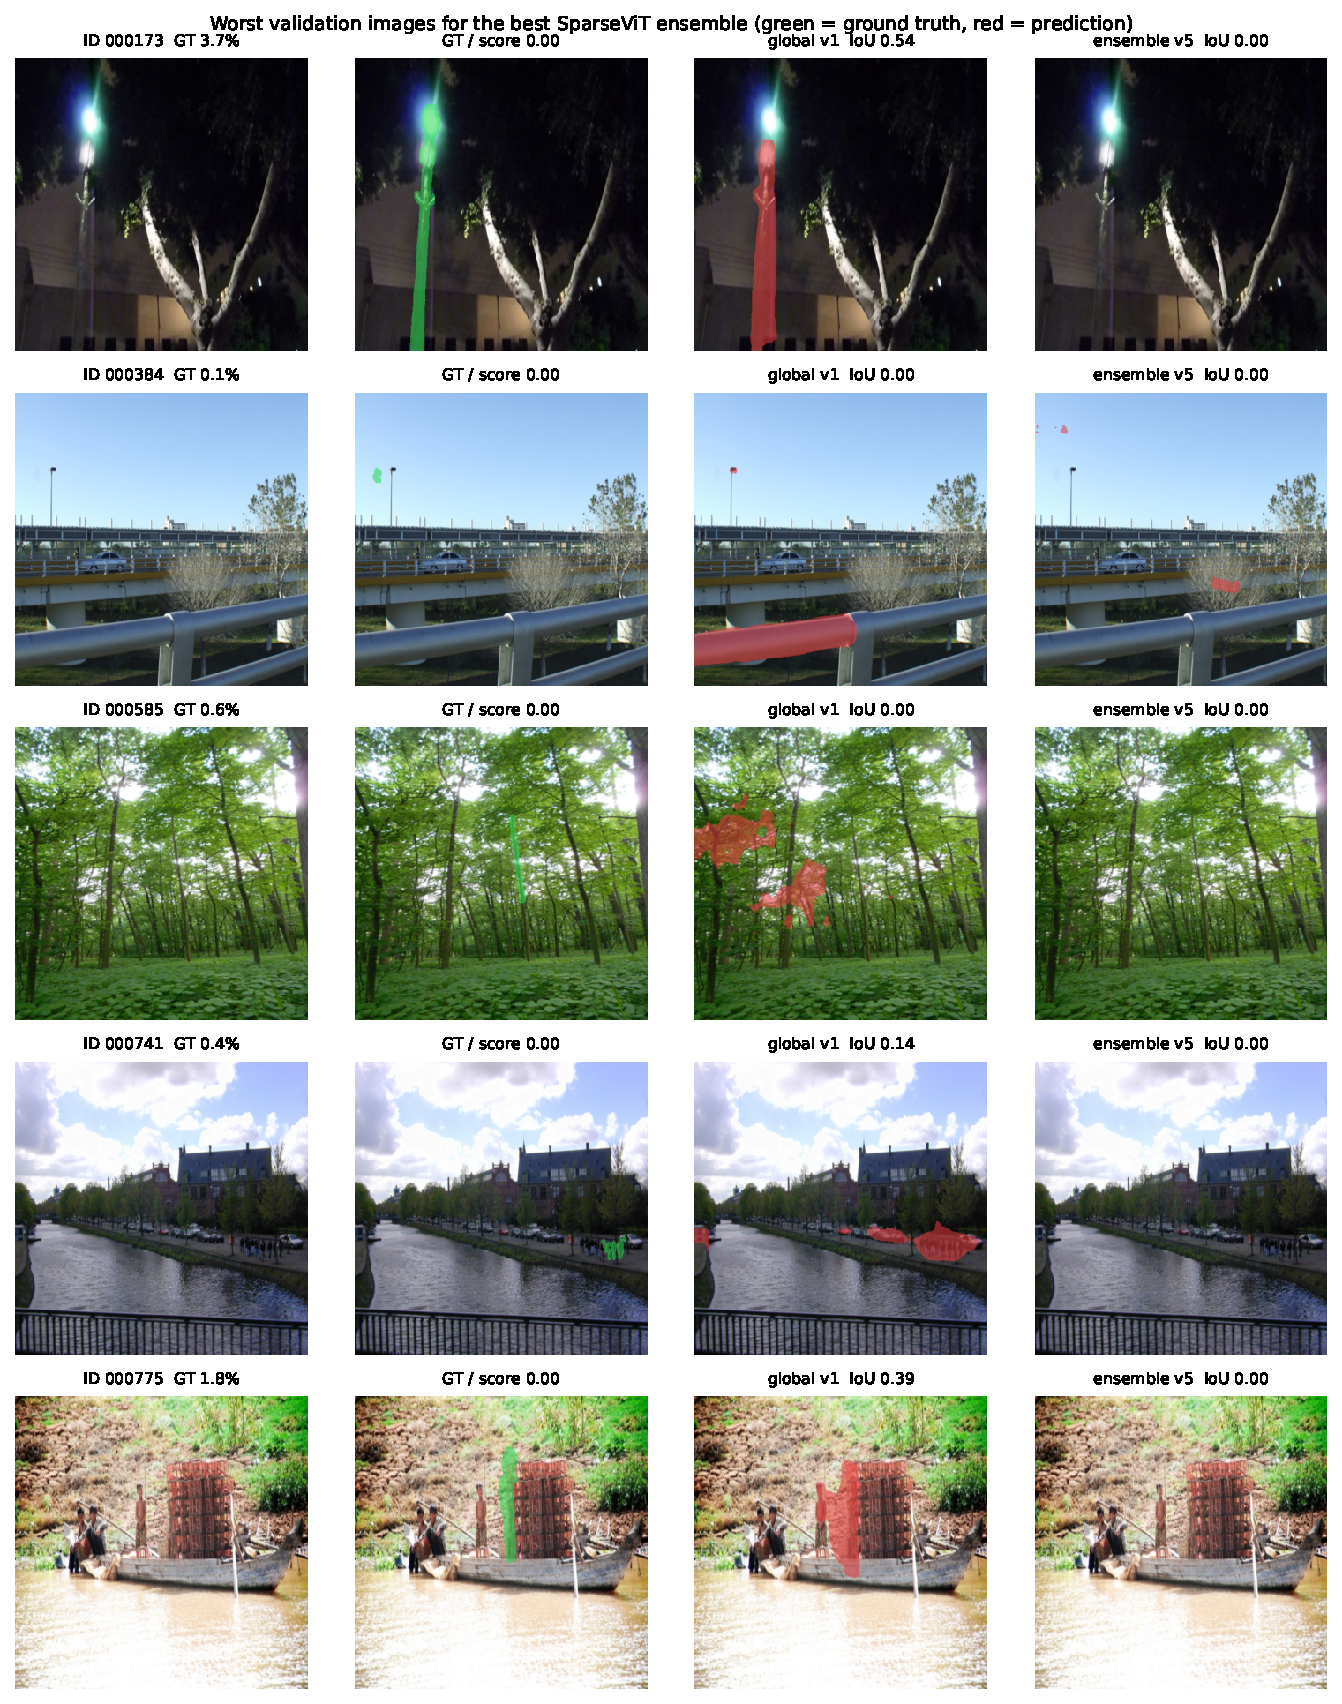
\includegraphics[width=.80\linewidth]{fig_val_errors}
\caption{Worst validation images: image, ground-truth overlay, global model, and ensemble (left to right).}
\label{fig:valerr}
\end{figure}

The final fusion has a different failure profile. Its predicted mean edited area on clean validation is $0.10605$ against $0.10661$ in the ground truth, and on the test set it is $0.11456$. Global area calibration is therefore not the problem. The worst clean-validation cases are small or low-contrast edits:
\begin{table}[htbp]\centering\footnotesize
\caption{Worst clean-validation images for the final fusion. ``Oracle'' is the best per-image threshold on the same probability map.}
\begin{tabular}{lrrrr}
\toprule ID & GT area & Score & Oracle & Comment \\
\midrule
003549 & 0.0265 & 0.7063 & 0.803 & threshold/coverage \\
003560 & 0.0121 & 0.7781 & 0.724 & small edit \\
004315 & 0.0199 & 0.7793 & 0.804 & boundary loss \\
003501 & 0.1052 & 0.7870 & 0.839 & ranking \\
000810 & -- & 0.8384 & -- & persistent failure \\
\bottomrule
\end{tabular}
\end{table}
For image $003549$, mean probability is $0.654$ on ground-truth pixels and $0.001$ on background. Decoding the submitted CSV and comparing it with the saved mask cache gives mean IoU $0.99997$, so RLE conversion does not contribute to these errors.

\section{Error analysis during training}
The full-data SparseViT run reached its best Score of $0.6690$ at epoch 9, with validation loss falling from $0.7164$ to $0.4740$ and training loss from $0.7964$ to $0.2493$. The last epoch was $0.0023$ below the best; a 20-epoch control on the 500/100 subset scored $0.5446$ against $0.5498$ for 10 epochs. With 5620 optimiser steps in 10 epochs, longer schedules added overfitting rather than coverage.

At the tuned threshold $0.20$, the pixel-level confusion matrix over 500 validation images is TP $=13{,}178{,}024$, FP $=3{,}658{,}621$, FN $=2{,}126{,}852$, TN $=112{,}108{,}503$, giving precision $0.7827$, recall $0.8610$, and specificity $0.9684$. The global branch predicts $13.3\%$ edited pixels against $11.7\%$ in the ground truth, so its false positives come from area over-prediction; the patch branch matches the prior at $11.8\%$. Fig.~\ref{fig:area} shows that Score falls mainly on small-edit images, where a fixed threshold either floods the mask or loses it entirely.
\begin{figure}[htbp]\centering
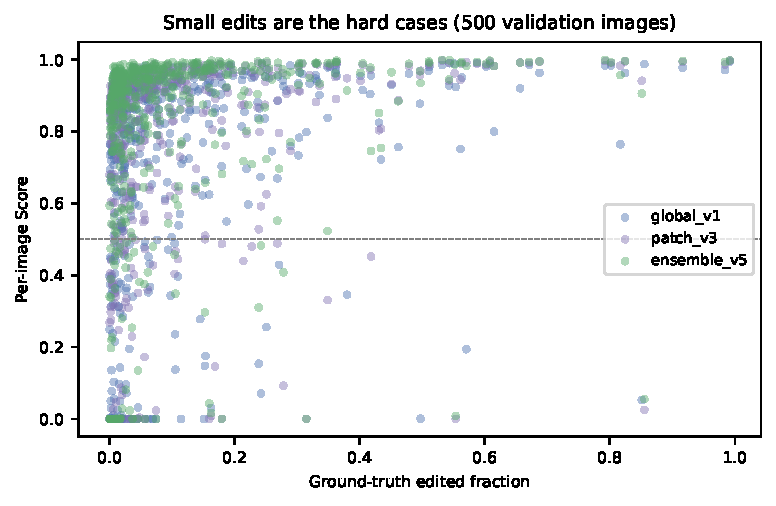
\includegraphics[width=.62\linewidth]{fig_area_vs_score}
\caption{Per-image Score versus ground-truth edited fraction for three SparseViT views.}
\label{fig:area}
\end{figure}

\section{The current probability family is saturated}
\label{sec:saturation}
\begin{table}[htbp]\centering\footnotesize
\caption{Clean-validation oracle bounds on 56 images.}
\begin{tabular}{lr}
\toprule Rule & Score \\
\midrule
Teacher + hysteresis & 0.95008 \\
Hard + hysteresis & 0.93977 \\
Current fusion & 0.953140 \\
Oracle per-image branch choice & 0.95387 \\
Oracle per-pixel branch choice & 0.95493 \\
\bottomrule
\end{tabular}
\end{table}
The per-pixel oracle exceeds the selected fusion by $0.00179$. No weighted average of the same two probability maps can close a $0.02819$ gap. The experiments below all failed to move the clean-validation proxy above $0.953140$.
\begin{table}[htbp]\centering\footnotesize
\caption{Negative results after the $0.92213$ baseline. Scores are Kaggle public Scores unless marked otherwise.}
\begin{tabular}{llr}
\toprule Intervention & Observation & Outcome \\
\midrule
Global/adaptive hysteresis, threshold sweeps & clean-val $0.953140$ & no gain \\
Component filtering, hole filling, closing, smoothing & Kaggle $0.92114$--$0.92209$ & below baseline \\
TTA16, 640px tiles, cross-overlap, 6-way/vote & clean-val $\le 0.953140$ & no gain \\
Pseudo-label self-training v2 & patch $0.91542$; fusion $0.953140$ & no gain \\
Full fine-tune \texttt{out\_ft\_full} & $0.91416$ vs hard student $0.92128$ & worse \\
From-scratch wide U-Net & below teacher family & rejected \\
\bottomrule
\end{tabular}
\end{table}
The proxy-to-Kaggle mapping is noisy: a clean-validation score of $0.93537$ mapped to $0.92213$, while $0.95314$ mapped to $0.93024$. A candidate needs a clear proxy gain before it uses submission quota.

\section{A new representation: literature and DINO tests}
\label{sec:dino}
Four lines of prior work motivated a representation change. DEAL-300K/MFPT (arXiv:2511.23377) reports that frozen visual foundation models plus frequency prompts improve diffusion-edit localisation, with DINOv2 stronger than EVA02. DinoLizer (arXiv:2511.20722) pairs frozen DINOv2 with a light head for inpainting detection. X-Edit (arXiv:2505.11753) uses inversion residuals and boundary-focused relevance, but needs captions and expensive inversion. SegFix (arXiv:2007.04269) shows that boundary pixels are less reliable than interior pixels and that model-agnostic boundary correction helps.

We tested DINOv2-S/14 in three forms on 448 native validation patches:
\begin{table}[htbp]\centering\footnotesize
\caption{DINO negative results against the historical teacher baseline.}
\begin{tabular}{lrr}
\toprule Variant & Patch-val Score & mIoU \\
\midrule
Standalone DINO-HF + light decoder & 0.46513 & 0.2359 \\
Frozen DINO + $1\times1$ linear probe & 0.47829 & 0.2827 \\
DINO injected into teacher bottleneck & 0.90527 & -- \\
Teacher baseline & 0.90953 & 0.8994 \\
\bottomrule
\end{tabular}
\end{table}
The standalone decoder produced nearly constant probabilities (mean $0.329$, standard deviation $0.086$), and the linear probe isolated the representation problem: frozen DINO tokens carry little localisation signal for this dataset. Injection into the teacher lost $0.00426$ against the baseline. We stopped this direction; the remaining error is a local texture and boundary problem that the native U-Net already captures.

\section{A complementary architecture: Mesorch with a pretrained local branch}
\label{sec:mesorch}
Mesorch (AAAI'25, arXiv:2412.13753) couples a CNN local branch on DCT high-frequency images with a transformer global branch on low-frequency images, decodes eight feature scales, and learns a pixel-wise softmax over them. We reimplemented DCT enhancement, the SegFormer-style global branch, the eight decoders and the weighting module from the paper; the local branch is the standard torchvision ImageNet-1K ConvNeXt-Tiny with its stem adapted from three to six channels (31.17M parameters). No implementation or weights were taken from the paper's authors.

Training used 9000 training and 1000 validation $512\times512$ patches, BCE+Dice loss, AdamW, and EMA. A small-batch run (800/160 patches) first confirmed convergence: Score rose from $0.581$ at step 200 to $0.81295$ at step 1200, versus $0.37$ for the same architecture from random initialisation. The full 20000-step run improved monotonically to \textbf{0.90983} patch-validation Score (teacher on the same split: $0.92052$), and the EMA checkpoint at step 20000 was retained.

On the 56-image clean-validation split with TTA8-style tiled inference, Mesorch alone scored $0.94712$, above teacher ($0.93914$) and hard ($0.94519$). Fusion with the hard model gave $0.95516$ at equal weights; adding the teacher term reduced the Score, so the selected recipe uses only Mesorch and hard. Four-way TTA with 64-pixel tile overlap was used for both branches. To avoid catastrophic false positives on test images where Mesorch disagreed strongly with both older models, an image-level consensus gate reverts to the previous canonical fusion when the Mesorch high-confidence area exceeds three times the larger of the teacher/hard areas plus $0.02$. The gate fires on 0/56 clean-validation images and 2/500 test images, and leaves the clean-validation Score unchanged.

The candidate was submitted to Kaggle and scored \textbf{0.94005} (ref $58928971$), a $0.00981$ improvement over the previous $0.93024$ entry. It is now the canonical submission. Error images with true positives in green, false positives in red and false negatives in blue are retained for the 20 worst clean-validation cases; the dominant remaining error is missed, low-contrast edited pixels.

\paragraph{Why boundary postprocessing was rejected.} Misclassified boundary pixels sit at low image gradients (mean $0.0454$) compared with correct boundaries ($0.0526$), so the errors are not displaced strong edges and there is nothing for a CRF or bilateral filter to snap to. Gaussian smoothing at $\sigma=0.5$--$2$ reduced the clean-validation Score from $0.95516$ to $0.95430$--$0.94351$, and bilateral variants to $0.94504$--$0.94687$; a hysteresis sweep gained only $0.0009$. Rendering the fused probability at full image resolution instead of $512\times512$ also hurt ($0.95219$ versus $0.95486$), so the remaining boundary uncertainty is intrinsic to these blended edits rather than an interpolation artefact.

\section{Current pipeline and the refiner experiment}
The current canonical recipe fuses Mesorch and hard-student probabilities at equal weight with TTA8, overlap 64, hysteresis high $0.92$ and low $0.38$, fallback threshold $0.5$, and the consensus gate above. The preceding teacher/hard recipe used teacher weight $0.4$ and hard weight $0.6$; its fallback reduced empty test masks from 11 to 3 without changing clean-validation Score.

The refiner uses three verified facts: the historical checkpoint reproduces the teacher cache exactly (mean absolute difference $0$), cached masks are true ground truth (patch/crop IoU $0.94$--$0.98$), and teacher probabilities can be regenerated with the same TTA8 settings. Its input is the RGB patch, the teacher probability, FFT high-pass and Sobel maps, and the probability-gradient magnitude. A width-16 U-Net predicts a refined probability from the true patch mask under BCE plus Dice loss on 9000 training patches, with 448 validation patches. The refined map replaces the teacher term in the existing $0.4/0.6$ fusion.

At the time of that experiment, promotion required patch-validation Score above $0.90953$, clean-validation fusion above $0.953140$, a two-column RLE dry-run, and a Kaggle Score strictly above $0.93024$. Until then the canonical file stays \texttt{submissions/best\_submission.csv}; any future candidate must now strictly exceed $0.94005$.

\textbf{Negative result (experiment run 2026-11-26).} We implemented and tested the residual variant, in which a zero-initialised head predicts a logit offset on top of the teacher logit, so step~0 is exactly the teacher. On an 800/160-patch smoke split (400/80 images), two seeds reached best-threshold Scores $0.91537$--$0.91539$ after 250 steps against teacher $0.91536$, although training loss fell from $0.467$ to $0.179$; the refiner consistently gained mIoU while losing mRecall. Re-evaluating the same checkpoint on all 1000 validation patches (500 images) gave $0.928925$, below the teacher's $0.928931$. The small apparent gain on 80 images was therefore noise and its sign flips on the full split. Gate~1 fails: we do not train the full model, do not build a test candidate, and keep the canonical $0.93024$ submission.

\section{Metric and reproduction}
For each image, $\mathrm{IoU}=TP/(TP+FP+FN)$, $\mathrm{Recall}=TP/(TP+FN)$, and $\mathrm{Score}=0.7\,\mathrm{mIoU}+0.3\,\mathrm{mRecall}$, averaged over images. Two empty masks count as 1; exactly one empty mask counts as 0. Probability caches are uint8 in $[0,255]$ and are divided by 255 before thresholding. RLE is column-major, 1-based, at original image dimensions; an empty mask is an empty string.

Rebuilding the PDF uses the committed JSON and figure evidence with \texttt{pdflatex}; full training and inference need CUDA and the supplied data. Checkpoint selection must use the full-image official Score, not patch-level Dice. The reproduction commands, training configurations, per-experiment table, and error JSON files remain in the repository and are unchanged by this revision.

Native pixels and metric-aligned validation remain necessary but are not sufficient: the teacher/hard family was within $0.0018$ of its clean-validation oracle and frozen semantic embeddings added nothing. A second architecture with complementary errors produced a confirmed Kaggle gain from $0.93024$ to $0.94005$. The residual refiner failed its patch-validation gate, and boundary or full-resolution postprocessing degraded the Score, so the remaining headroom to the top-3 cutoff must come from stronger or more diverse learned signals rather than from postprocessing the current probabilities.
\end{document}
